% !TEX TS-program = pdflatex
% !TEX encoding = UTF-8 Unicode

% This is a simple template for a LaTeX document using the "article" class.
% See "book", "report", "letter" for other types of document.

\documentclass[11pt]{article} % use larger type; default would be 10pt

\usepackage[utf8]{inputenc} % set input encoding (not needed with XeLaTeX)

\usepackage{graphicx} %package to manage images
\graphicspath{{images/} }

%%% Examples of Article customizations
% These packages are optional, depending whether you want the features they provide.
% See the LaTeX Companion or other references for full information.

%%% PAGE DIMENSIONS
\usepackage{geometry} % to change the page dimensions
\geometry{a4paper} % or letterpaper (US) or a5paper or....
% \geometry{margin=2in} % for example, change the margins to 2 inches all round
% \geometry{landscape} % set up the page for landscape
%   read geometry.pdf for detailed page layout information

\usepackage{graphicx} % support the \includegraphics command and options

% \usepackage[parfill]{parskip} % Activate to begin paragraphs with an empty line rather than an indent

%%% PACKAGES
\usepackage{booktabs} % for much better looking tables
\usepackage{array} % for better arrays (eg matrices) in maths
\usepackage{paralist} % very flexible & customisable lists (eg. enumerate/itemize, etc.)
\usepackage{verbatim} % adds environment for commenting out blocks of text & for better verbatim
\usepackage{subfig} % make it possible to include more than one captioned figure/table in a single float
% These packages are all incorporated in the memoir class to one degree or another...

%%% HEADERS & FOOTERS
\usepackage{fancyhdr} % This should be set AFTER setting up the page geometry
\pagestyle{fancy} % options: empty , plain , fancy
\renewcommand{\headrulewidth}{0pt} % customise the layout...
\lhead{}\chead{}\rhead{}
\lfoot{}\cfoot{\thepage}\rfoot{}

%%% SECTION TITLE APPEARANCE
\usepackage{sectsty}
\allsectionsfont{\sffamily\mdseries\upshape} % (See the fntguide.pdf for font help)
% (This matches ConTeXt defaults)

%font sezioni ecc
\usepackage{titlesec}

\titleformat{\section} {\normalfont\large\bfseries\centering}{\thesection}{1em}{}
\titleformat{\subsection} {\normalfont\large}{\thesubsection}{1em}{}
\titleformat{\subsubsection} {\normalfont\normalsize}{\thesubsubsection}{1em}{}
\titleformat{\paragraph}[runin] {\normalfont\normalsize}{\theparagraph}{1em}{}
\titleformat{\subparagraph}[runin] {\normalfont\normalsize}{\thesubparagraph}{1em}{}

%%% ToC (table of contents) APPEARANCE
\usepackage[nottoc,notlof,notlot]{tocbibind} % Put the bibliography in the ToC
\usepackage[titles,subfigure]{tocloft} % Alter the style of the Table of Contents
\renewcommand{\cftsecfont}{\rmfamily\mdseries\upshape}
\renewcommand{\cftsecpagefont}{\rmfamily\mdseries\upshape} % No bold!

%%% END Article customizations

%%% The "real" document content comes below...

\title{TSPC 4-bit Full Adder}
\author{Francesco Morgillo\\3810105}
%\date{} % Activate to display a given date or no date (if empty),
         % otherwise the current date is printed 

\begin{document}
\maketitle

\section{Obiettivi del progetto }
Si presenta il progetto di design di un full-adder a 4 bit con tecnologia MOS 0.12 $\mu m$ e logica TSPC (true single phase clock). 
Il Full Adder presenta quattro ingressi: due word a 4 bit di cui eseguire la somma ($a_{0},b_{0}$), un $CARRY IN$ ($ c_{0}$) e un ingresso dedicato al clock ($\phi$).
Le uscite del circuito sono i segnali di $SUM$ e $CARRY$.
Lo schema del circuito di una cella a 1 bit del full-adder è riposrtato in Figura \ref{fig:Schematic}
\begin{figure}[h!]
  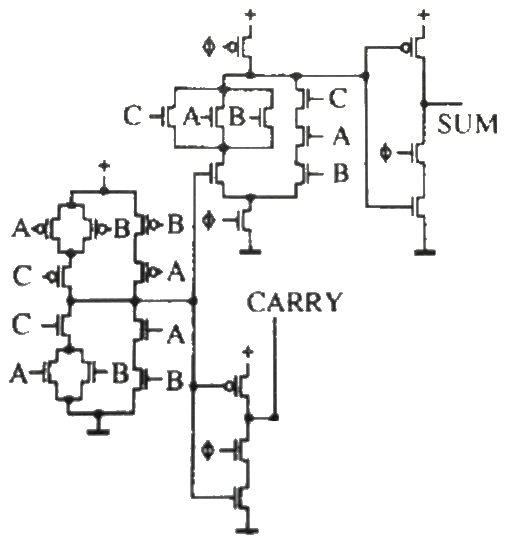
\includegraphics[scale=0.75]{Schematic.png}
  \caption{Circuito full-adder TSPC, 1 bit}
  \label{fig:Schematic}
\end{figure}

\

\subsection{Specifiche del Progetto}
Per la realizzazione del circuito sono richieste l'utilizzo di tecnologia MOS a 0.12 $\mu m$, un'alimentazione a $1.2V$, frequenza di lavoro $2GHz$,  carico capacitivo di $100fF$ e una dimensione della cella con altezza massima di 68$\lambda$.

\section{Logica TSPC}
La logica TSPC prevede l'utilizzo di un blocco di logica statica e di un segnale di clock che temporizza uno stadio latch. Si hanno due fasi differenti: una di precarica (quando $\phi=0$) ed una di valutazione (quando $\phi=1$). Il segnale di uscita va considerato in fase di valutazione.

\section{Dimensionamento}
Sono state considerate le specifiche relative alla frequenza di funzionamento e al carico per ottenere le dimensioni dei transistor, nei vari stadi.  
E' necessario innanzitutto calcolare le dimensioni di $W_{n}$ dello stadio finale. Calcolando il carico equivalente di ogni stadio, si ottiene a ritroso il valore di $W_{n}$ di ogni stadio.
Le dimensioni $W_{n}$ si ottengono con la formula seguente:

\begin{equation} 
\frac{W_{n}}{L}=\frac{2CV_{dd}}{\
 \mu_{n}C_{ox}(V_{gs}-V_{th})^2}
\end{equation}
Dove:\mbox{}\\

\begin{tabular}{|ll|}
\hline
$V_{gs}$ & $1.20V$ \\
$C$ & $100fF$ \\
$\tau$ & 250ps\\
$\mu_{n}$ & $0.06$  $\frac{fF}{m^2}$  \\
$C_{ox}$ & $0.01725$ $\frac{m^2}{Vs}$  \\
$V_{gs} - V_{th}$ & $0.8V$ \\
\hline
\end{tabular}
\mbox{}\\
\\
Partendo dal terzo stadio si applica la formula e considerando il vincolo di tecnologia $L= 120 nm$ di ottiene un rapporto $\frac {W_{n}}{L}= 1.4486$.
Si approssima all'intero successivo visto che larghezza  $W_{n}$ non può che essere un multiplo intero di L :   $W_{n}=2L= 240nm$.
Per un transistor $p$ si dovrà triplicare questo valore per via della minor mobilità degli elettroni nel substrato $P$, quindi $W_{p}=3W_{n}= 720nm$.

Per quanto riguarda il secondo stadio è necessario considerare la capacità equivalente che esso vede sul terzo stadio.
La capacità equivalente viene calcolata come segue :
\begin{equation}
C_{G}= C_{ox}W_{n}L+C_{ox}W_{p}L= 2.93fF
\end{equation}
Il valore del carico da pilotare è abbastanza piccolo per poter utilizzare dei transistor a dimensione minima ($W_{n}=120 nm$, $W_{p}=3W_{n}= 360nm$)
Lo stesso ragionamento porta a scegliere dei transistor a dimensione minima anche nel primo stadio. 

\section{Realizzazione e simulazione}

Il circuito è stato quindi realizzato con \emph{Microwind} e in Figura \ref{fig:Layout1} ne è riportato il layout.
L'area compresa fra le rail di alimentazione è di $66\lambda$ x $167 \lambda$.

\begin{figure}[h!]
  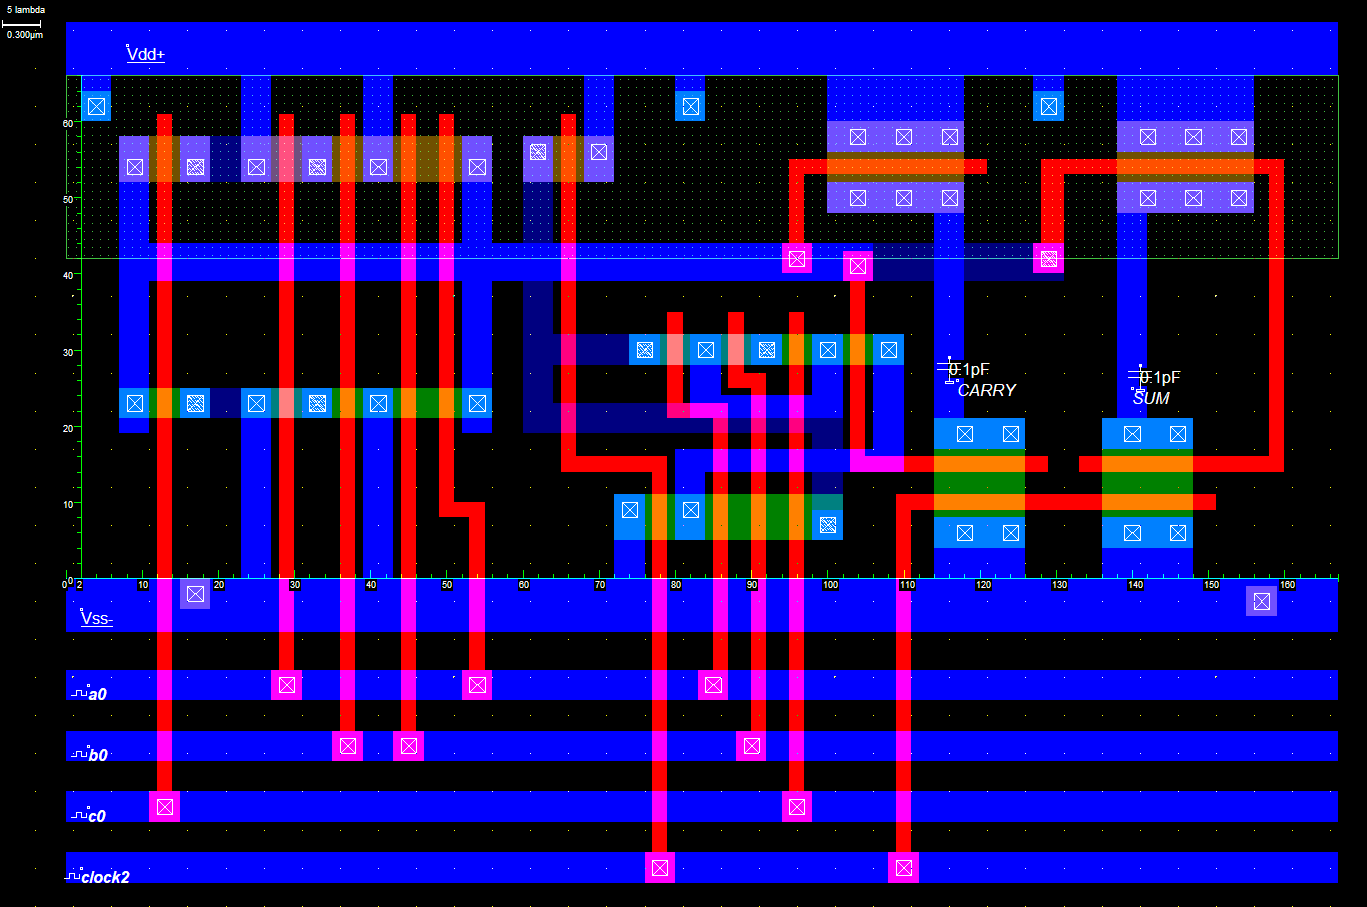
\includegraphics[width=\linewidth]{Layout1.png}
  \caption{Layout Full-Adder}
  \label{fig:Layout1}
\end{figure}

\begin{figure}[h!]
  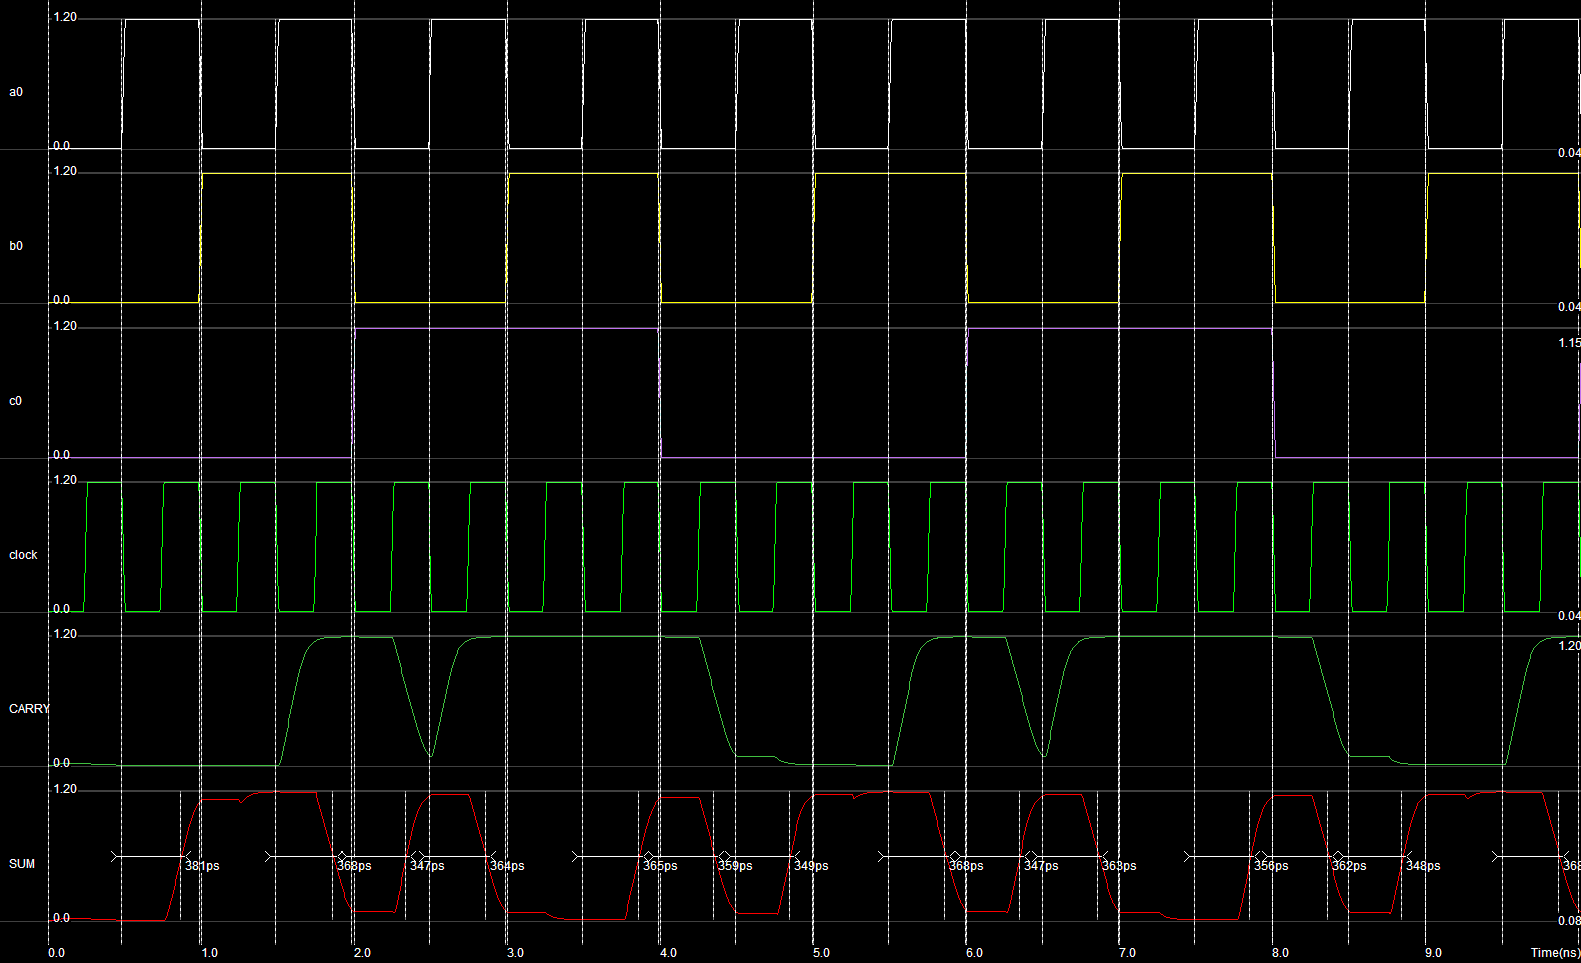
\includegraphics[width=\linewidth]{Micro1.png}
  \caption{Simulazione in Microwind}
  \label{fig:Micro1}
\end{figure}

\begin{figure} [h!]
  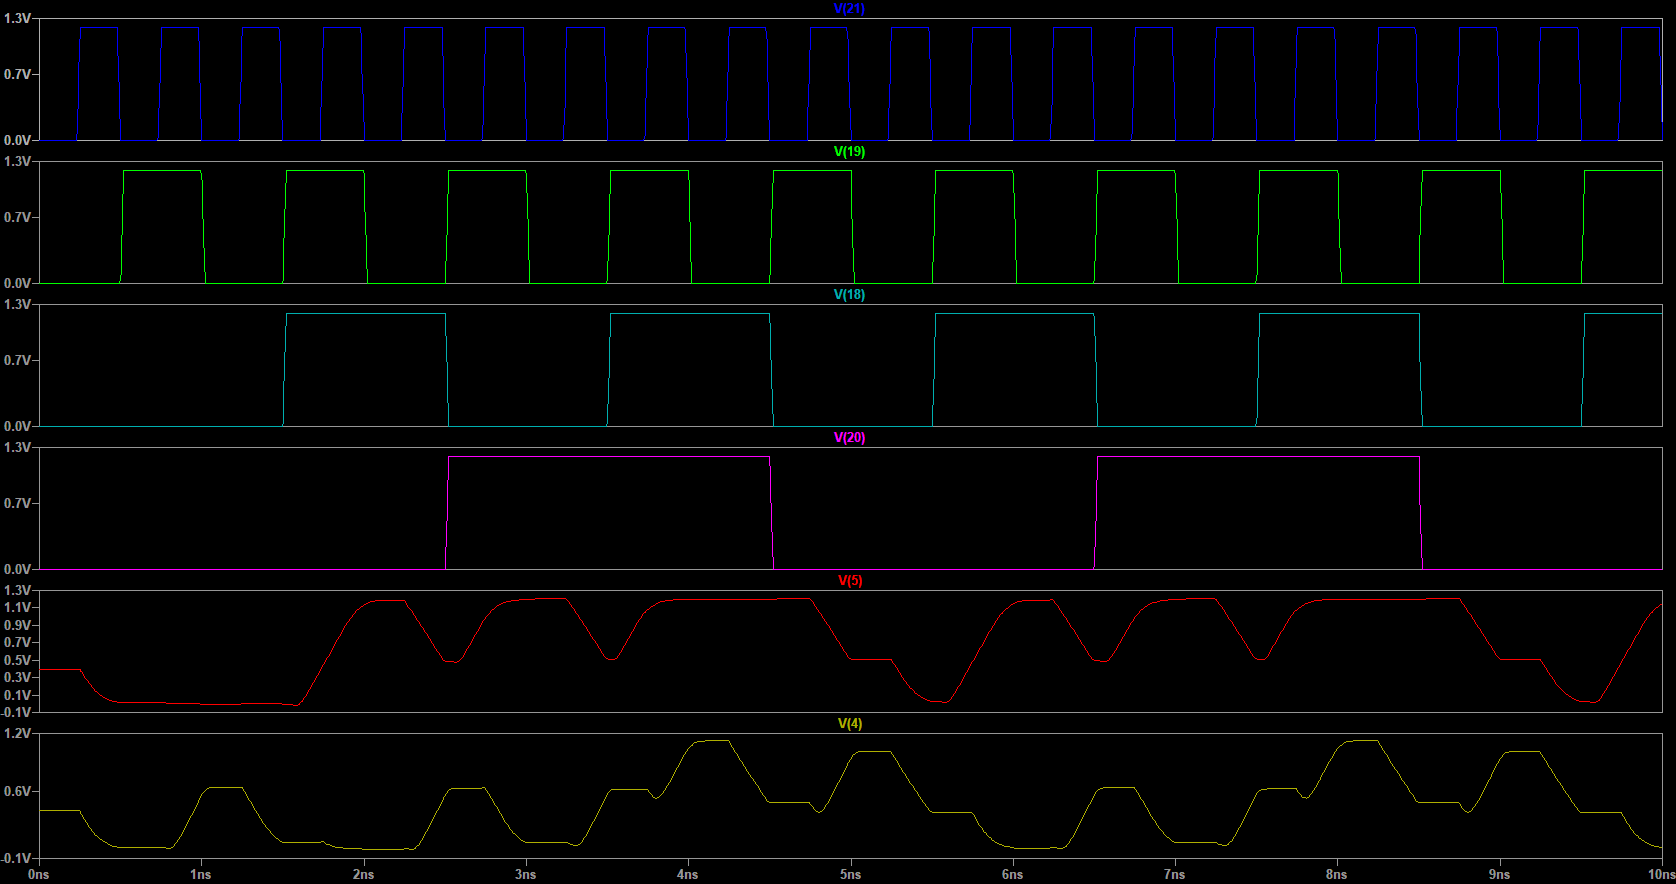
\includegraphics[width=\linewidth]{Vecchio.png}
  \caption{Simulazione in LTSpice}
  \label{fig:LT1}
\end{figure}


Dalla simulazione del circuito, svolta in ambiente \emph{Microwind}, si nota che le uscite del circuito non sono abbastanza veloci nella commutazione oppure non raggiungono valori di tensione adeguati.


\begin {table} [h!]
\begin{tabular}{|c|c|c|c|}
\hline
$ Clock$ $\phi$ & $V(19)$\\
\hline
$A0$ & $V(20)$ \\
\hline
$B0$ & $V(21)$\\
\hline
$C0$ &  $V(18)$  \\
\hline
$CARRY$ & $V(5)$  \\
\hline
$SUM$ & $V(4)$ \\
\hline
\end{tabular}
\caption{Tabella dei segnali di Figura \ref{fig:LT1}}
\label{table:1}
\end{table}

Importando la netlist del layout su \emph{LT Spice} si può osservare più nel dettaglio tali ritardi(Figura \ref{fig:LT1}).


Osservando per esempio la prima transizione del segnale $SUM$, si nota che la tensione non raggiunge, nel tempo necessario la tensione sufficiente per ottenere un valore logico alto.
Oppure nel caso del segnale di $CARRY$, sempre seguendone la prima transizione, si nota il ritardo di salita ma anche la difficoltà nel raggiungere lo zero prima che sopraggiunga una nuova variazione.

I segnali della Figura \ref{fig:LT1}  sono riportati nella tabella  \ref{table:1}.


Questo comportamento indesiderato viene corretto effettuando un nuovo dimensionamento, procedendo con il graduale aumento della larghezza dei transistor coinvolti, partendo da quelli dello stadio finale.
\newline 
Di fatto aumentando la dimensione dei transistor dell'ultimo stadio, si aumenta la corrente per caricare le capacità di carico.
Seguendo lo stesso ragionamento gli stadi precedenti vedono una capacità di carico dovuta al gate dello stadio che pilotano: si ridimensioneranno anche questi stadi di conseguenza.
\newpage
\section{Ridimensionamento}
Il layout del circuito è stato quindi ridimensionato ed è riportato in Figura \ref{fig:Layout2}.


 \begin{figure}[h]
  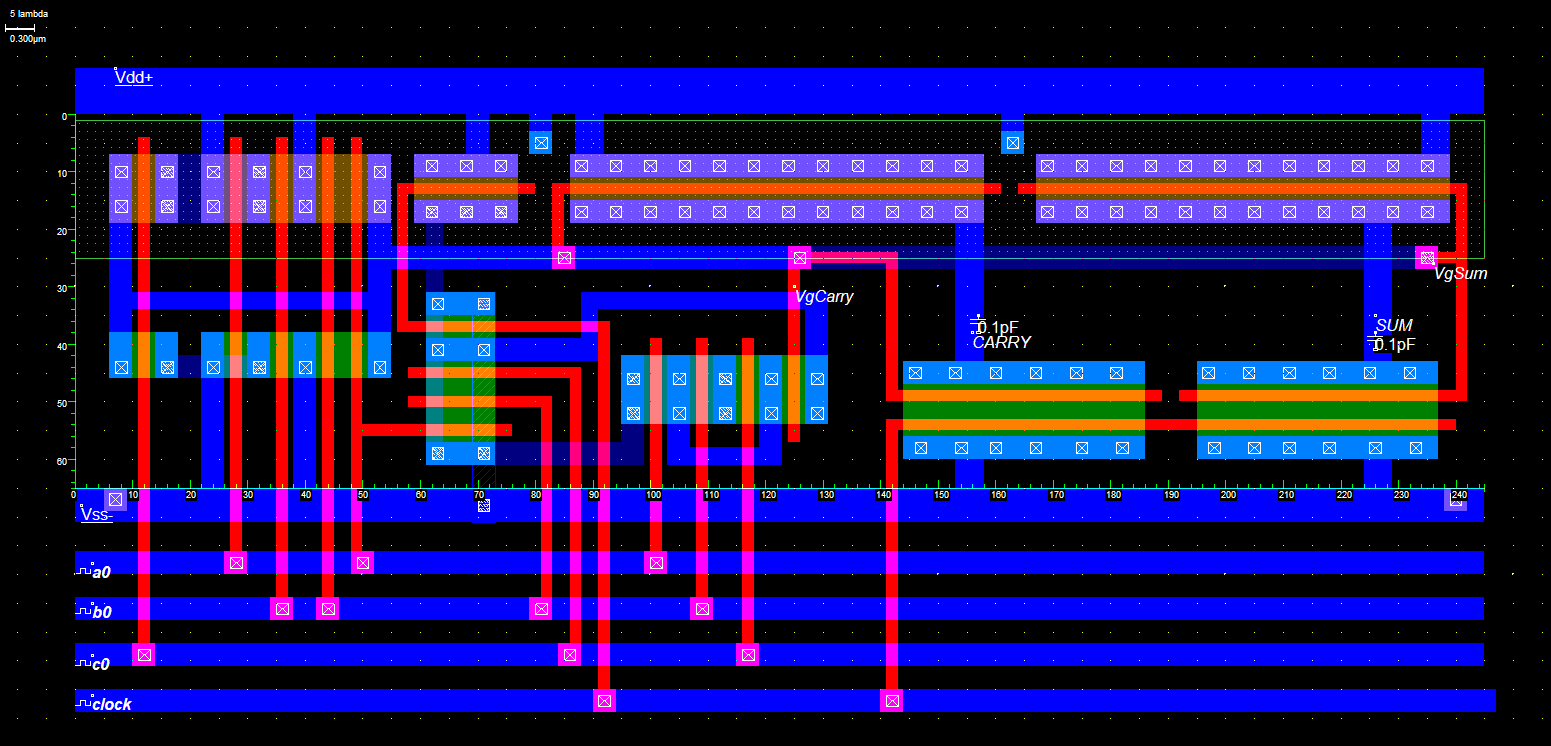
\includegraphics[width=\linewidth]{Layout2.png}
  \caption{Layout Full-Adder modificato}
  \label{fig:Layout2}
\end{figure}
 
I MOS dell'ultimo stadio sono stati notevolmente ingranditi e di conseguenza anche quelli degli stadi precedenti.
L'area compresa fra le rail di alimentazione è di $65\lambda$ x $245 \lambda$.
Dai risultati della simulazione su \emph{LT Spice} si nota come i segnali siano ora notevolmente più definiti e con un timing migliorato.
In particolare, il segnale $SUM$ questa volta raggiunge un valore di tensione adeguato per essere considerato "$HIGH$" rispettando i tempi di valuazione e pre-carica imposti dal clock.

\begin{figure}[h!]
  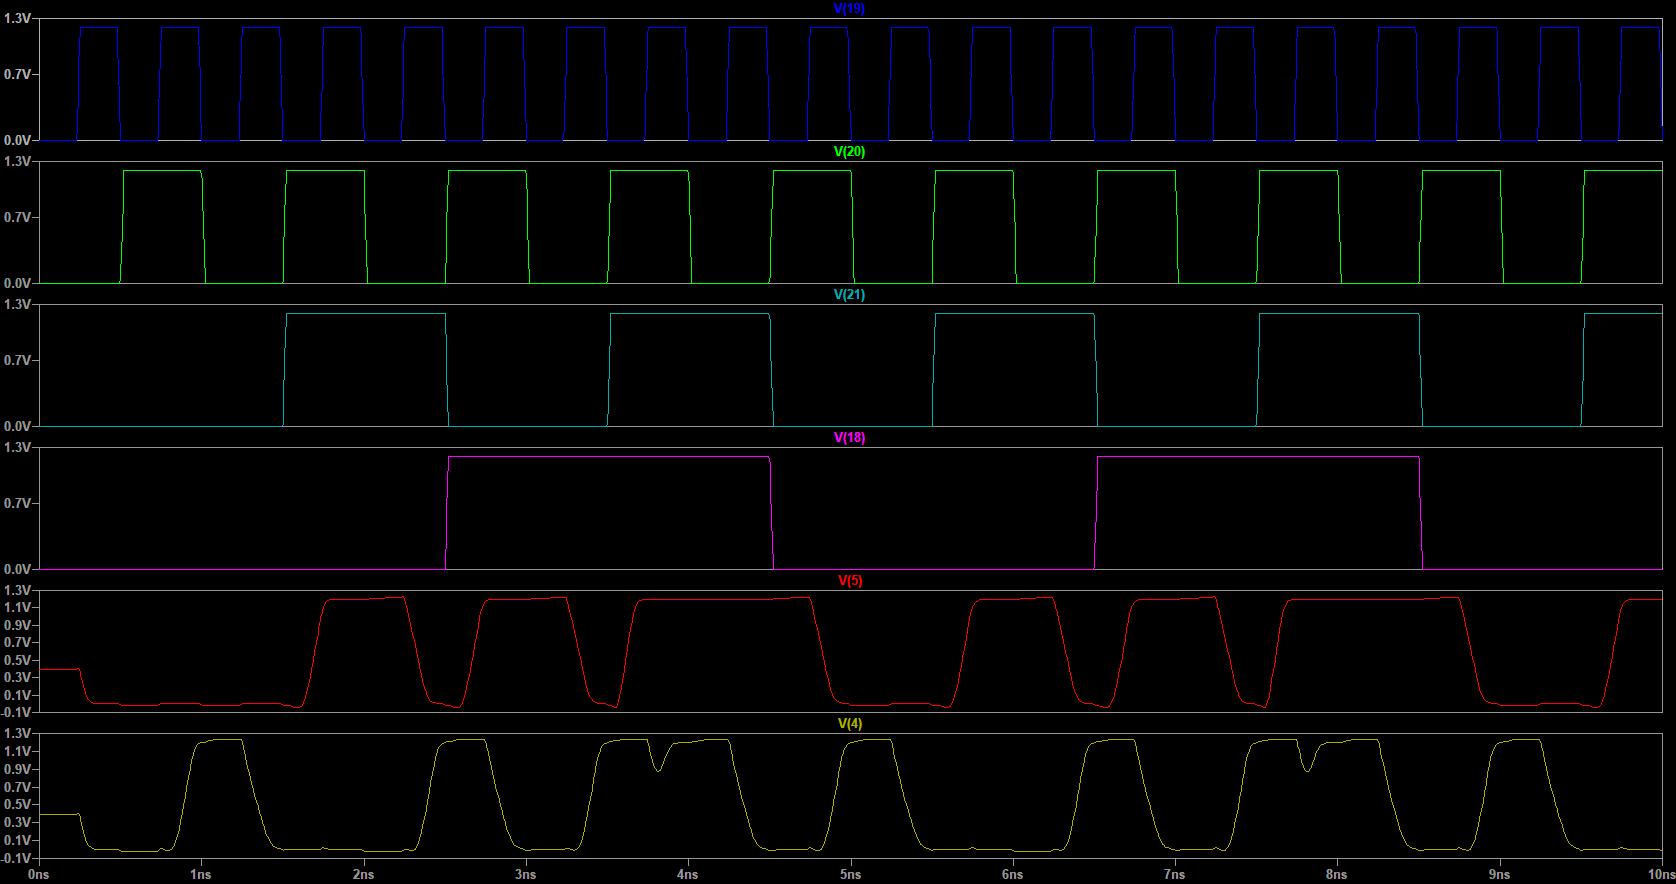
\includegraphics[width=\linewidth]{LT2.png}
  \caption{Simulazione in LT SPice del layout corretto}
  \label{fig:LT2}
\end{figure}

Allo stesso modo il segnale $CARRY$ raggiunge il valore basso con una pendenza maggiore, quindi anch'esso in tempo per una nuova transizione.
\clearpage

\section{Potenza assorbita}
Sempre utilizzando \emph{LT Spice} si è ottenuta la traccia del prodotto $V_{dd}*I$ a rappresentare la Potenza istantanea assorbita dal circuito (riportata in Figura \ref{fig:Power}).
\newline
Sempre tramite \emph{LT Spice} si è ottenuto una misura del valor medio pari a $305.18 $  $\mu W$

 \begin{figure}[h!]
  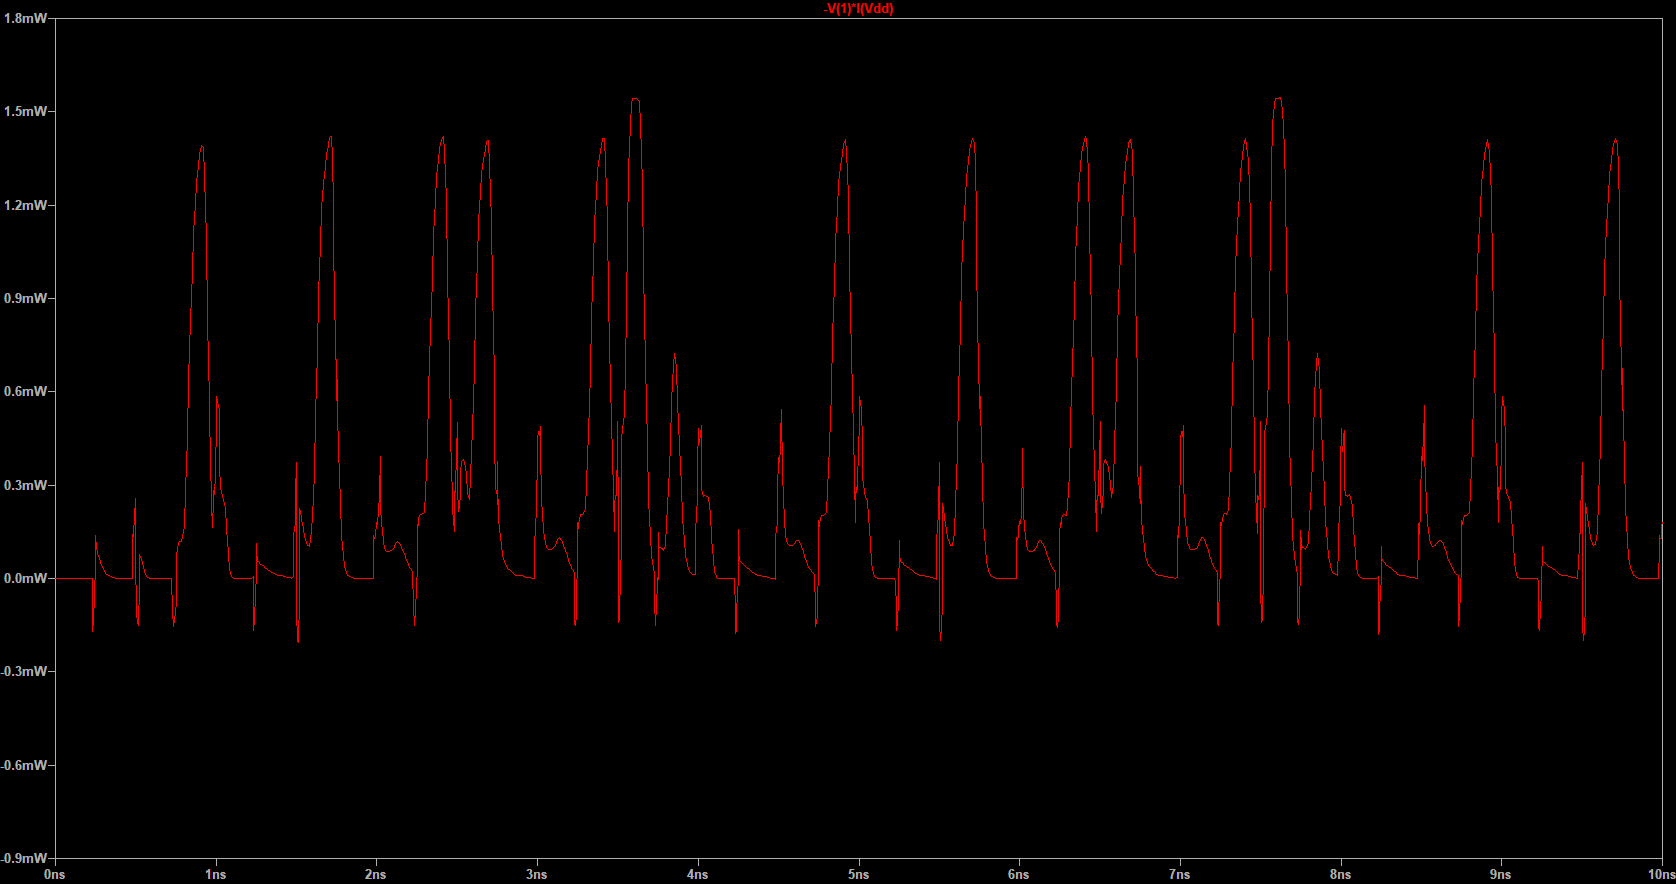
\includegraphics[width=\linewidth]{power.png}
  \caption{Potenza istantanea}
  \label{fig:Power}
\end{figure}
\end{document}